\documentclass[main.tex]{subfiles}
% \numberwithin{equation}{section}
% \setcounter{section}{10}
% \numberwithin{figure}{section}
\begin{document}

\section{Conservation of Charge}


\subsection{Millikan's Oil Drop Experiment} \label{e8Ie5P}

The American physicist Robert Millikan (1868-1953) and his student Harvey Fletcher (1884-1981) were the first to make a relatively accurate measurement of the fundamental unit of charge on the electron. They designed what is now a classic experiment performed by students. The Millikan oil-drop experiment is shown on the right. The basic idea of the experiment is that a fine oil mist is sprayed between two plates that can be charged with a known amount of opposite charge. Some oil drops accumulate some excess negative charge when being sprayed and are attracted to the positive charge of the upper plate and repelled by the negative charge on the lower plate. By tuning the charge on these plates until the weight of the oil drop is balanced by the electric forces, the experimenter may determine to a high degree of precision the oil drop's net charge.


\vspace{1em}
\cyanhrule

\subsection*{\ref{e8Ie5P} Exercises}

\textbf{\ref{6YGfUm}--\ref{Q68N4Y}} Watch ``Charge of an Electron: Millikan's Oil Drop Experiment'' by Tyler DeWitt on YouTube (\href{https://youtu.be/2HhaQtvICe8}{click here}), then answer the exercises below.

\begin{exercise} \label{6YGfUm}
    In what year did Millikan and Fletcher conduct the oil drop experiment?
\end{exercise}

\begin{exercise}
    J.~J.~Thompson discovered the electron, the negatively charged particle, in the year \rule{2cm}{0.15mm}.
\end{exercise}

\begin{exercise}
    The Millikan's oil drop experiment involves balancing tiny drops of oil by using gravity and \rule{2cm}{0.15mm}.
\end{exercise}


\begin{exercise}
    Two parts of the equipment used by Millikan are the \rule{2cm}{0.15mm} and the \rule{2cm}{0.15mm}.
\end{exercise}

\begin{exercise}
    Which force acts downward on the oil drop?
\end{exercise}

\begin{exercise}
    Which plate--the positively or the negatively charged---will the positive oil drop be attracted to? Explain.
\end{exercise}

\begin{exercise}
    What force pushes the oil drop in the opposite direction of gravity?
\end{exercise}

\begin{exercise}
    When the voltage is too HIGH, the oil drop moves \rule{2cm}{0.15mm}.
\end{exercise}

\begin{exercise}
    When the voltage is too LOW, the oil drop moves \rule{2cm}{0.15mm}.
\end{exercise}

\begin{exercise}
    What happens to the oil drop when the voltage through the apparatus is just right?
\end{exercise}

\begin{exercise}
    The force of gravity on the drop depends only on the \rule{2cm}{0.15mm} of the drop.
\end{exercise}

\begin{exercise}
    What 2 factors does the force of electricity on the drop depend on?
\end{exercise}

\begin{exercise} \label{Q68N4Y}
    What is the charge of 1 electron?
\end{exercise}

\subsection{Discovery of Electric charge} \label{DicxAf}
\Gls{electric charge} is a property of matter that causes objects to attract or repel each other. Electric charge comes in two varieties: positive ($+$) and negative ($-$). Like charges repel each other, and unlike charges attract each other. Thus, two positive charges repel each other, as do two negative charges. A positive charge and a negative charge attract each other.
\vspace{1em}

When various materials are rubbed together in controlled ways, certain combinations of materials always result in a net charge of one type on one material and a net charge of the opposite type on the other material. By convention, we call one type of charge positive and the other type negative. For example, when glass is rubbed with silk, the glass becomes positively charged and the silk negatively charged. Because the glass and silk have opposite charges, they attract one another like clothes that have rubbed together in a dryer. Two glass rods rubbed with silk in this manner will repel one another, because each rod has positive charge on it. Similarly, two silk cloths rubbed in this manner will repel each other, because both cloths have negative charge.

\vspace{1em}



It took scientists a long time to discover what lay behind these two types of charges. The word electric itself comes from the Greek word \textit{elektron} for amber, because the ancient Greeks noticed that amber, when rubbed by fur, attracts dry straw. Almost 2,000 years later, in 1897, the English physicist J.~J.~Thomson and French physicist Jean Perrin, were studying the mysterious cathode rays that were known at the time to consist of particles smaller than the smallest atom. Perrin showed that cathode rays actually carried negative electrical charge. Later, Thomson's work led him to declare, ``I can see no escape from the conclusion that [cathode rays] are charges of negative electricity carried by particles of matter.''
Science had in fact discovered the particle that carries the fundamental unit of negative electrical charge. We now know this particle as the \gls{electron}.
\vspace{1em}


Atoms, however, were known to be electrically neutral, which means that they carry the same amount of positive and negative charge, so their net charge is zero. Because electrons are negative, some other part of the atom must contain positive charge. Thomson put forth what is called the \textit{plum pudding model}, in which he described atoms as being made of thousands of electrons swimming around in a nebulous mass of positive charge. His student, Ernest Rutherford, originally believed that this model was correct and used it (along with other models) to try to understand the results of his experiments bombarding gold foils with alpha particles (i.e., helium atoms stripped of their electrons). The results, however, did not confirm Thomson's model but rather destroyed it! Rutherford found that most of the space occupied by the gold atoms was actually empty and that almost all of the matter of each atom was concentrated into a tiny, extremely dense nucleus. The atomic nucleus was later found to contain particles called protons.  Each \gls{proton} carries a unit of positive electric charge.


\vspace{1em}

Protons and electrons are thus the fundamental particles that carry electric charge. Each proton carries one unit of positive charge, and each electron carries one unit of negative charge. To the best precision that modern technology can provide, the charge carried by a proton is \textit{exactly} the opposite of that carried by an electron. The SI unit for electric charge is the \gls{coulomb} (abbreviated as C), which is named after the French physicist Charles Augustin de Coulomb, who studied the force between charged objects. The name for the magnitude of the charge on 1 proton or 1 electron is the \gls{elementary charge}, which is the fundamental unit of electric change and has a value of 

\begin{equation}
    e = \qty{1.602e-19}{C}
\end{equation}

Thus the proton carries a charge ($q$) of $q_\text{p} = +e$ and the electron one of $q_\text{e} = -e$. The elementary charge is the smallest possible unit of charge.

\subsection*{\ref{DicxAf} Exercises}

\begin{exercise}
    \href{https://phet.colorado.edu/en/simulations/balloons-and-static-electricity/about}{Click here} to access the PhET Simulation ``Balloons and Static Electricity.'' Spend a few minutes exploring this simulation to gain understanding of the transfer of electric charge.
\end{exercise}

\begin{exercise}
    What is electric charge?
\end{exercise}

\begin{exercise}
    Electric charge comes in only two types. What are those types?
\end{exercise}

\begin{exercise}
    Like charges \rule{2cm}{0.15mm}, and opposite charges \rule{2cm}{0.15mm}.
\end{exercise}

\begin{exercise}
    When you rub a glass rod with a piece of silk, electric charge is transferred. Which object acquires a positive charge? and which a negative charge?
\end{exercise}

\begin{exercise}
    What is the origin of the word ``electric''?
\end{exercise}

\begin{exercise}
    In what year was the electron discovered?
\end{exercise}

\begin{exercise}
    What does it mean when an atom or an object (like a glass rod) is electrically \textit{neutral}?
\end{exercise}

\begin{exercise}
    What did J.~J.~Thomson call his early model of the atom?
\end{exercise}

\begin{exercise}
    What astonishing discovery did Ernest Rutherford make about the atom to disprove Thompson's model?
\end{exercise}

\begin{exercise}
    What is the particle that carries the positive electric charge?
\end{exercise}

\begin{exercise}
    The SI unit of electric charge is the \rule{2cm}{0.15mm}.
\end{exercise}

\begin{exercise}
    Write the value and the unit of the \gls{elementary charge}---the smallest and most fundamental unit of electric charge, which is carried by the proton or negatively by the electron.
\end{exercise}

\begin{exercise}
    What is the charge of 1 electron?
\end{exercise}

\begin{exercise}
    What is the charge of 1 proton?
\end{exercise}

\cyanhrule

\subsection{Transfer of Electric Charge} \label{XFJNUr}

Protons are stuck to the atom. Electrons are free to transfer away from atoms and to other objects. When electrons are transferred, charge is transferred. An object containing equal amounts of protons and electrons is electrically neutral: its net charge is zero. An object with either an excess or a deficit of electrons will acquire a net electrical charge. An object with 1 excess electron will have a charge of $-e$; with 2 excess electrons, a charge of $-2e$; with 3 excess electrons, a charge of $-3e$, and so on. In general, an object with $n$ excess electrons has a net electric charge ($q$) of

\begin{equation} \label{Dabfyz}
    q = - ne \hspace{1em} \text{(electron excess)}
\end{equation}

\begin{center}
    \begin{tabular}{cl|cc}
    \hline
    \textbf{Symbol} & \textbf{Quantity} & \textbf{SI Base Unit} & \textbf{Unit Symbol}  \\
    \hline\hline
    \rule{0pt}{2.5ex}
        $q$ & net charge & coulomb & \si{\coulomb}\\
        $n$ & number of excess electrons & (none) & (none) \\
        $e$ & elementary charge & coulomb & \si{\coulomb} \\
    \hline
    \end{tabular}
\end{center}

\begin{example}
    After rubbing on a shirt, a balloon acquires 25 excess electrons. What is the electric charge on the balloon?
\end{example}

\Solution We are given the number of excess electrons: $n = 25$. We know the elementary charge (on each electron): $e = \SI{1.6e-19}{C}$. The unknown is the electric charge on the balloon: $q =\ ?$. By Equation~\ref{Dabfyz}, electric charge is

\begin{equation*}
    q = - n e = -25\,(\num{1.6e-19}) = \SI{-4.0e-18}{C}
\end{equation*}

\cyanhrule

\begin{multicols}{2}

\subsection*{\ref{XFJNUr} Exercises}

\textbf{\ref{IyrMKh}--\ref{VKqxLG}} Do a Google search for the \href{https://phet.colorado.edu/en/simulations/balloons-and-static-electricity/about}{PhET Simulation} called \texttt{Balloons and Static Electricity}. Rub 1 balloon against the shirt. Observe how it can stick to the shirt and to the wall. Click \texttt[red]{Reset Balloon}.
Next, rub 1 balloon against one half of the shirt, and the other balloon against the other half of the shirt. Observe how the balloons are attracted to the shirt but repelled by each other.

\begin{exercise} \label{IyrMKh}
    What happens to the electrons ($-$) when you rub the shirt against the balloon?
\end{exercise}

% \begin{exercise}
%     In your own words, define the terms \textit{excess}, \textit{deficit}, and \textit{neutral}. (While you may search a dictionary for these terms, you must use your own words to define them.) 
% \end{exercise}



\begin{exercise}
    What does it mean that a balloon has an ``electron excess''?
\end{exercise}

\begin{exercise}
    What does it mean that the wool shirt has an ``electron deficit'?
\end{exercise}

\begin{exercise}
    Why is the balloon attracted to the shirt?
\end{exercise}

\begin{exercise} \label{VKqxLG}
    Why are the balloons repelled by each other?
\end{exercise}

\cyanhrule

\begin{exercise} \label{9U7zJj}
    Look at Equation (\ref{Dabfyz}) for the charge on an object that has an electron excess. What equation would you use to calculate the net charge on an object that has an electron \textit{deficit}?
\end{exercise}

\begin{exercise} \label{gEsEJ7}
    A rain cloud discharges 5 billion billion excess electrons through a lightning strike. What is the total charge carried by the lightning strike?
\end{exercise}



\begin{exercise} \label{d3zygU}
    What is the charge on a dust particle that contains five thousand excess electrons?
\end{exercise}

\begin{exercise} \label{ERkfIH}
    If an electric fence delivers \SI{4.2e16}{} electrons to a person who touches it, what is the electric charge transferred to the person?
\end{exercise}

\begin{exercise} \label{9qwZGy}
    How many protons are required to make \SI{2.89}{C} of charge?
\end{exercise}

\end{multicols}

\cyanhrule

\subsection{Powers of 10} \label{tdVujC}

Powers of 10 and scientific notation are powerful ways to write very large and very small numbers. Powers of 10 work as follows:

\begin{equation*}
    10^0 = 1\ , \quad 10^1 = 10\ , \quad 10^2 = 100\ , \quad 10^3 = \SI{1000}{}\ , \qquad 10^6 = \SI{1000000}{}\ \qquad 10^{11} = \SI{100000000000}{}
\end{equation*}

Likewise,

\begin{equation*}
    10^{-1} = \frac{1}{10} = 0.1\ , \quad
    10^{-2} = \frac{1}{100} = \SI{0.01}{}\ , \quad 
    10^{-5} = \frac{1}{\SI{100000}{}} = 0.000\,01\ ,\qquad
    10^{-8} = \frac{1}{\num{100000000}} = 0.000\,000\,01
\end{equation*}

In this unit, when working with scientific notation and powers of ten, we will often be dividing powers of 10. For example, $10^2/10^{-3}$. Here we may apply the following quotient property.


\begin{example}
    Calculate $10^7/10^4$ by hand.
\end{example}

\Solution This fraction is worked out as follows:

\begin{equation*}
    \frac{10^7}{10^4} = 10^{7-4} = 10^3
\end{equation*}

\begin{example}
    Calculate $10^2/10^{-3}$ by hand.
\end{example}

\Solution The solution is

\begin{equation*}
    \frac{10^2}{10^{-3}} = 10^{2 - (-3)} = 10^5
\end{equation*}

\cyanhrule
\vspace{1em}

The following property reminds us how to compute such fractions generally.

\begin{mdframed}[backgroundcolor=black!10]
    \textbf{Quotient Property for Exponents.} If $m$ and $n$ are integers, then

    \begin{equation} \label{6Kyqsn}
        \frac{10^m}{10^n} = 10^{m-n}
    \end{equation}
\end{mdframed}







\begin{example}
    The net charge on a microscopic piece of silver is \SI{-5}{nC}. (a) What does the silver piece have: electron excess or electron deficit? (b) How many electrons are in excess/deficit compared to neutrality?
\end{example}

\Solution (a) Since the silver's charge is negative, it must have excess electrons (more electrons than protons).

\vspace{1em}

(b) The metric prefix nC means \textit{nano}coulomb, where \textit{nano} represents $10^{-9}$. Therefore, the net charge is $q = \SI{-5}{nC} = \SI{-5e-9}{C}$. As usual, the elementary charge is $e= \SI{1.602e-19}{C}$. By Equation (\ref{Dabfyz}),

\begin{equation*}
    q = -ne
\end{equation*}

Substituting known values, while omitting units, leads to

\begin{equation*}
     \num{-5e-9} = - n\,(\num{1.602e-19})
\end{equation*}

We solve this equation for the number of electrons as follows:

\begin{align*}
    \textbf{Write $n$ on left} \qquad & - n\,(\SI{1.602e-19}{}) = \SI{-5e-9}{}\\[1ex]
    \textbf{Divide by \SI{-1.602e-19}{}} \qquad & \frac{- n\,(\cancel{\SI{1.602e-19}{}})}{\redminus \textcolor{red}{\cancel{\SI{1.602e-19}{}}}} = \frac{\SI{-5e-9}{}}{\redminus \textcolor{red}{\SI{1.602e-19}{}}}\\[1ex]
    \textbf{Simplify} \qquad & n = \frac{\qty{5e-9}{}}{\qty{1.602e-19}{}}\\[1ex]
    \textbf{Separate factors} \qquad & \frac{5}{1.602} \times \frac{10^{-9}}{10^{-19}}\\[1ex]
    \textbf{Use Quotient Property (Eq.~\ref{6Kyqsn})} \qquad & \frac{5}{1.602} \times 10^{-9 - (-19)}\\[1ex]
    \textbf{Simplify} \qquad & \frac{5}{1.602} \times 10^{10}\\[1ex]
    \textbf{Divide} \qquad & \SI{3.12e10}{}
\end{align*}

Therefore, $n = \SI{3.12e10}{}$, so there are about 30 billion excess electrons on the piece of silver.

\vspace{1em}
\cyanhrule

\subsection*{\ref{tdVujC} Exercises}

\begin{exercise} \label{994stj}
    Vera's wool shirt acquires a net charge of \SI{3.5}{nC}. (a) Does the shirt have an electron excess or an electron deficit? (b) How many electrons are in excess or deficit from neutrality?
\end{exercise}

\begin{exercise} \label{IRX4Zr}
    Calculate the number of excess electrons on a metal sphere that has an electric charge of \qty{-0.003}{C}.
\end{exercise}


% \begin{example} \label{Se9sG1}
% How many protons are required to make \SI{1.00}{C} of charge?
% \end{example}

% \Solution Each proton carries $+\SI{1.602e-19}{C}$. The number of protons, $n$, required to 1 coulomb of charge is found by

% \begin{equation*}
%     n = \SI{1.00}{C} \times \frac{\text{1 proton}}{\SI{1.602e-19}{C}} = \SI{6.25e18}{}\,\text{protons}
% \end{equation*}


\cyanhrule

\subsection{Coulomb's Law} \label{fKC05f}

Two charges always exert a \href{https://phet.colorado.edu/en/simulations/coulombs-law}{mutual force} on each other. The charges may be a proton and an electron, or they may be macroscopic objects like a balloon and a shirt. Opposite charges generate an attractive force, and like charges, a repulsive one. 


\def\distanceA{5}
\def\distanceR{2}

\begin{center}
\begin{tikzpicture}
\begin{axis}[width=8cm,height=3.7cm,
    clip=false,
    xmin=-0.5,xmax=6,ymin=-0.6,ymax=1.2,
    axis line style={draw=none},
    ticks=none,    
]
    \fill (0,0) circle (3pt);
    \draw (0,0) circle (6mm) node[above=6mm] {$q_1\,(+)$};
    \draw[->,thick] (0,0) -- ++(axis direction cs: 2,0) node[below] {$F$};

    \begin{scope}[xshift=\distanceA*0.99 cm]
        \fill (0,0) circle (3pt);
        \draw (0,0) circle (6mm) node[above=6mm] {$q_2\,(-)$};
        \draw[->,thick] (0,0) -- ++(axis direction cs: -2,0) node[below] {$F$};
    \end{scope}

    \draw[<->,dashed] (0,0.2) -- ++(axis direction cs: \distanceA,0);
    \node[above=6pt] at (\distanceA/2,0) {$r$};
    \node[above=1cm] at (\distanceA/2,0) {\textbf{Attractive}};
\end{axis}
\end{tikzpicture}%
\hspace{1cm}
\begin{tikzpicture}
\begin{axis}[width=8cm,height=3.7cm,
    clip=false,
    xmin=-2.1,xmax=4,ymin=-0.6,ymax=1.2,
    axis line style={draw=none},
    ticks=none,    
]
    \fill (0,0) circle (3pt);
    \draw (0,0) circle (6mm) node[above=6mm] {$q_3\,(+)$};
    \draw[->,thick] (0,0) -- ++(axis direction cs: -2,0) node[below] {$F$};
    
    \begin{scope}[xshift=\distanceR*1.07 cm]
        \fill (0,0) circle (3pt);
        \draw (0,0) circle (6mm) node[above=6mm] {$q_4\,(+)$};
        \draw[->,thick] (0,0) -- ++(axis direction cs: +2,0) node[below] {$F$};
    \end{scope}
    
    \draw[<->,dashed] (0,0.2) -- ++(axis direction cs: \distanceR,0);
    \node[above=6pt] at (\distanceR/2,0) {$r$};
    \node[above=1cm] at (\distanceR/2,0) {\textbf{Repulsive}};
\end{axis}
\end{tikzpicture}
\end{center}

This force is called the electrostatic force. Its magnitude is given by \gls{Coulomb's law}:

\begin{equation} \label{TjSj69}
    F = \frac{k|q_1 q_2|}{r^2}    
\end{equation}

where $k$ is the Coulomb's constant, $q_1$ and $q_2$ are the charges of each object, and $r$ is the distance between the objects. Coulomb's law implies that object 1 exerts an electric force on object 2 that is equal in magnitude to the force that object 2 exerts on object 1.
\vspace{1em}

The Coulomb's constant, $k$, is a physical constant---a universal value that does not change and applies for all applications of Coulomb's law. Its magnitude is given by

\begin{equation}
    k = \SI{8.99e9}{N \cdot m^2/C^2}
\end{equation}

but may be approximated as \SI{9e9}{N \cdot m^2/C^2}. Note that $|q_1 q_2|$ is the \href{https://openstax.org/books/elementary-algebra-2e/pages/1-3-add-and-subtract-integers}{absolute value} of the product of $q_1$ and $q_2$; the absolute value of a number is always greater than or equal to zero.

\begin{center}
\begin{tabular}{cl|cc}
\hline
\textbf{Symbol} & \textbf{Quantity} & \textbf{SI Base Unit} & \textbf{Unit Symbol}  \\
\hline\hline
\rule{0pt}{2.5ex}
    $F$ & electric force & newton & \si{\newton}\\
    $k$ & Coulomb constant & (\textit{see} $\rightarrow$) & \SI{}{N \cdot m^2/C^2}\\
    $q_1$ & charge of object 1 & coulomb & \si{\coulomb}\\
    $q_2$ & charge of object 2 & coulomb & \si{\coulomb} \\
    $r$ & distance & meter & \si{\meter} \\
\hline
\end{tabular}
\end{center}

\clearpage
\begin{mdframed}[backgroundcolor=black!10]
\textbf{Metric prefix:} The metric prefix ``micro'' (µ) means one-millionth:

\begin{equation*}
    1\,\text{µ} = \frac{1}{\SI{1000000}{}} =\SI{1e-6}{}
\end{equation*}

So, a micro coulomb means $\SI{1}{\micro C} = \SI{1e-6}{C}$.
\end{mdframed}

\begin{example} \label{e3NF5s}
Two spheres with charges \SI{-4}{\micro C} and \SI{8}{\micro C} are separated by \SI{3}{cm}. (a) Is the electric force between the objects attractive or repulsive? (b) What is the magnitude of the electric force between them?
\end{example}

\Solution (a) Because the charges have opposite charges, they will attract. (b) We are given the charges of two objects and the distance between them. Converting the given quantities of charge and distance to SI base units of coulombs and meters, we express the quantities as

\begin{equation*}
    q_1 = \SI{-4}{\micro C} = \SI{-4e-6}{C} 
    \qquad \text{and} \qquad
    q_2 = \SI{8}{\micro C} = \SI{8e-6}{C}
\end{equation*}

and $r = \SI{3}{cm} = \SI{0.03}{m}$. The diagram of the charges is shown below:

\begin{center}
\begin{tikzpicture}
\begin{axis}[width=8cm,height=3.7cm,
    clip=false,
    xmin=-0.5,xmax=6,ymin=-0.6,ymax=1.2,
    axis line style={draw=none},
    ticks=none,    
]
    \fill (0,0) circle (3pt);
    \draw (0,0) circle (6mm) node[above=6mm] {$\SI{-4e-6}{C}$};
    \draw[->,thick] (0,0) -- ++(axis direction cs: 2,0) node[below] {$F$};

    \begin{scope}[xshift=\distanceA*0.99 cm]
        \fill (0,0) circle (3pt);
        \draw (0,0) circle (6mm) node[above=6mm] {$\SI{8e-6}{C}$};
        \draw[->,thick] (0,0) -- ++(axis direction cs: -2,0) node[below] {$F$};
    \end{scope}

    \draw[<->,dashed] (0,0.2) -- ++(axis direction cs: \distanceA,0);
    \node[above=6pt] at (\distanceA/2,0) {\SI{0.03}{m}};
\end{axis}
\end{tikzpicture}
\end{center}

By Coulomb's law, Eq.~(\ref{TjSj69}), the electric force between these charged spheres is

\begin{equation*}
    F = \frac{k q_1 q_2}{r^2} = \frac{\left(\SI{8.99e9}{}\right) \left|\left(\SI{-4e-6}{}\right) \left(\SI{8e-6}{}\right)\right|}{\left(\SI{0.03}{}\right)^2} =
    \SI{319.6}{N}
\end{equation*}

\cyanhrule

\subsection*{\ref{fKC05f} Exercises}

% \begin{multicols}{2}
\begin{exercise}
    Google the \textit{PhET Simulation} called \texttt{Coulomb's law} (or \href{https://phet.colorado.edu/en/simulations/coulombs-law}{click here}). Press \texttt{Play}, and select the \texttt{Macro Scale} panel. This simulation helps you understand Coulomb's law. (a) How does the magnitude and direction of the force on $q_1$ by $q_2$ compare to that of the force on $q_2$ by $q_1$? (b) What changes in the simulation cause the magnitude of the forces to increase? (c) What changes cause the magnitude of the force to decrease? (d) What changes cause the direction of the forces to change?
\end{exercise}

\begin{exercise} \label{z4pMlx}
Two objects with charges \SI{7}{\micro C} and \SI{5}{\micro C} are separated by \SI{2}{cm}. (a) Is the electric force between them attractive or repulsive? (b) What is the magnitude of the electric force between the spheres?
\end{exercise}

\begin{exercise} \label{TPIAio}
    Two metallic spheres with charges \SI{-7}{\micro C} and \SI{5}{\micro C} are separated by \SI{2}{cm}. (a) Do the spheres attract each other, or do they repel? (b) What is the magnitude of the electric force between the spheres?
\end{exercise}

\begin{exercise} \label{mJu5SD}
    As shown below, two charges are placed near each other. (a) Are they attracted or repulsed? (b) What is the magnitude of the electric force between the charges?
    \vspace{-1em}
    
\begin{center}
\begin{tikzpicture}
\begin{axis}[width=8cm,height=3.7cm,
    clip=false,
    xmin=-2.1,xmax=4,ymin=-0.6,ymax=1.2,
    axis line style={draw=none},
    ticks=none,    
]
    \fill (0,0) circle (2pt);
    \draw (0,0) circle (6mm) node[above=6mm] {\SI{8}{\micro C}};
    
    \begin{scope}[xshift=\distanceR*1.07 cm]
        \fill (0,0) circle (2pt);
        \draw (0,0) circle (6mm) node[above=6mm] {\SI{9}{\micro C}};
    \end{scope}
    
    \draw[<->,dashed] (0,0.2) -- ++(axis direction cs: \distanceR,0);
    \node[above=6pt] at (\distanceR/2,0) {\SI{6}{cm}};
\end{axis}
\end{tikzpicture}
\end{center}
\end{exercise}

\begin{exercise} \label{NqU30G}
(a) Are the charges below attracted or repulsed by each other? (b) Calculate the electrostatic force between them.
\vspace{-1em}

\begin{center}
\begin{tikzpicture}
\begin{axis}[width=8cm,height=3.7cm,
    clip=false,
    xmin=-2.1,xmax=4,ymin=-0.6,ymax=1.2,
    axis line style={draw=none},
    ticks=none,    
]
    \fill (0,0) circle (2pt);
    \draw (0,0) circle (6mm) node[above=6mm] {\SI{-3.2}{\micro C}};
    
    \begin{scope}[xshift=\distanceR*1.07 cm]
        \fill (0,0) circle (2pt);
        \draw (0,0) circle (6mm) node[above=6mm] {\SI{-2.5}{\micro C}};
    \end{scope}
    
    \draw[<->,dashed] (0,0.2) -- ++(axis direction cs: \distanceR,0);
    \node[above=6pt] at (\distanceR/2,0) {\SI{1.4}{cm}};
\end{axis}
\end{tikzpicture}
\end{center}
\end{exercise}

\begin{exercise} \label{S2QW5m}
When the two opposite charges shown below are placed near each other, the magnitude of the electrostatic force is \SI{44}{N}. What is the distance between the charges?

\begin{center}
\begin{tikzpicture}
\begin{axis}[width=8cm,height=3.7cm,
    clip=false,
    xmin=-0.5,xmax=6,ymin=-0.6,ymax=1.2,
    axis line style={draw=none},
    ticks=none,    
]
    \fill (0,0) circle (3pt);
    \draw (0,0) circle (6mm) node[above=6mm] {\SI{-680}{\micro C}};
    \draw[->,thick] (0,0) -- ++(axis direction cs: 2,0) node[below] {$\SI{44}{N}$};

    \begin{scope}[xshift=\distanceA*0.99 cm]
        \fill (0,0) circle (3pt);
        \draw (0,0) circle (6mm) node[above=6mm] {\SI{180}{\micro C}};
        \draw[->,thick] (0,0) -- ++(axis direction cs: -2,0); %node[below] {$F$};
    \end{scope}

    \draw[<->,dashed] (0,0.2) -- ++(axis direction cs: \distanceA,0);
    \node[above=6pt] at (\distanceA/2,0) {$r =\ ?$};
\end{axis}
\end{tikzpicture}
\end{center}
\end{exercise}

% \end{multicols}

\cyanhrule
\clearpage
\begin{example}
    A \SI{-50}{\micro C} charge and a \SI{95}{\micro C} one are separated by an unknown distance. If the electrostatic force between the charges is \SI{18.9}{N}, what is the distance between the charges?
\end{example}

\begin{center}
\begin{tikzpicture}
\begin{axis}[width=8cm,height=3.7cm,
    clip=false,
    xmin=-0.5,xmax=6,ymin=-0.6,ymax=1.2,
    axis line style={draw=none},
    ticks=none,    
]
    \fill (0,0) circle (3pt);
    \draw (0,0) circle (6mm) node[above=6mm] {$q_1$};
    \draw[->,thick] (0,0) -- ++(axis direction cs: 2,0) node[below] {$F$};

    \begin{scope}[xshift=\distanceA*0.99 cm]
        \fill (0,0) circle (3pt);
        \draw (0,0) circle (6mm) node[above=6mm] {$q_2$};
        \draw[->,thick] (0,0) -- ++(axis direction cs: -2,0) node[below] {$F$};
    \end{scope}

    \draw[<->,dashed] (0,0.2) -- ++(axis direction cs: \distanceA,0);
    \node[above=6pt] at (\distanceA/2,0) {$r =\ ?$};
\end{axis}
\end{tikzpicture}
\end{center}

\Solution We are given two charges and the electrostatic force: $q_1 = \SI{-50}{\micro C} = \qty{-50e-6}{C}$, $q_2 = \SI{95}{\micro C} = \qty{95e-6}{C}$, $F = \SI{18.9}{N}$. We want to find the separation distance between the charges: $r =\ ?$. These quantities are related by Coulomb's law:

\begin{equation*}
    F = \frac{k |q_1 q_2|}{r^2}\ ,
\end{equation*}

where Coulomb's constant is

\begin{equation*}
    k = \SI{8.99e9}{N \cdot m^2/C^2}
\end{equation*}

Plugging in these values into Coulomb's law leads to 

\begin{equation*}
    18.9 = \frac{(\num{8.99e9}) \left|(\qty{-50e-6}{C})(\qty{95e-6}{C})\right|}{r^2}
\end{equation*} 

This equation is solved for distance $r$ as follows:

\begin{align*}
    \textbf{Multiply across numerator} \qquad & 18.9 = \frac{\textcolor{red}{42.7}}{r^2}\\[1ex]
    \textbf{Multiply by $r^2$} \qquad & 18.9\,\textcolor{red}{r^2} = \frac{42.7}{\cancel{r^2}} \cdot \textcolor{red}{\cancel{r^2}}\\[1ex]
    \textbf{Simplify} \qquad & 18.9\,r^2 = 42.7\\[1ex]
    \textbf{Divide by 18.9} \qquad & \frac{\cancel{18.9}\,r^2}{\textcolor{red}{\cancel{18.9}}} = \frac{42.7}{\textcolor{red}{18.9}}\\[1ex]
    \textbf{Simplify} \qquad & r^2 = 2.26\\
    \textbf{Take square root} \qquad & r = \sqrt{2.26}\\[1ex]
    \textbf{Compute square root} \qquad & r = \qty{1.50}{m}\\ 
\end{align*}

\cyanhrule

\subsection*{\ref{fKC05f} Exercises (cont.)}

\begin{exercise} \label{clmO0M}
    A \SI{-48}{\micro C} charge and a \SI{55}{\micro C} one are separated by an unknown distance. If the electrostatic force between the charges is \SI{8.2}{N}, what is the distance between the charges?
\end{exercise}

\begin{exercise} \label{TrRzFe}
Calculate the distance between the charges below if the force $F$ is \qty{7.52e-3}{N}.

\begin{center}
\begin{tikzpicture}
\begin{axis}[width=8cm,height=3.7cm,
    clip=false,
    xmin=-0.5,xmax=6,ymin=-0.6,ymax=1.2,
    axis line style={draw=none},
    ticks=none,    
]
    \fill (0,0) circle (3pt);
    \draw (0,0) circle (6mm) node[above=6mm] {\SI{-860}{\micro C}};
    \draw[->,thick] (0,0) -- ++(axis direction cs: 2,0) node[below] {$F$};

    \begin{scope}[xshift=\distanceA*0.99 cm]
        \fill (0,0) circle (3pt);
        \draw (0,0) circle (6mm) node[above=6mm] {\SI{420}{\micro C}};
        \draw[->,thick] (0,0) -- ++(axis direction cs: -2,0); %node[below] {$F$};
    \end{scope}

    \draw[<->,dashed] (0,0.2) -- ++(axis direction cs: \distanceA,0);
    \node[above=6pt] at (\distanceA/2,0) {$r =\ ?$};
\end{axis}
\end{tikzpicture}
\end{center}
\end{exercise}

\begin{exercise} \label{bpbHHg}
    When a 0.0066-coulomb charge is placed near a 0.0044-coulomb one, they experience a mutual repulsive force with a magnitude of 74 newtons. What is the distance between the charges?
\end{exercise}


\begin{exercise} \label{DOuqpT}
    Solve Exercise \ref{TrRzFe} analytically, which means using
    only algebraic symbols and manipulation, and no numbers. Your result should be an equation solved for $r$ in terms of $F$, $k$, $q_1$, and $q_2$.
\end{exercise}
\clearpage

\subsection{Factor of Change Method} \label{MeMuHN}

The \gls{factor of change method} allows you to calculate proportional changes in the electrostatic force with proportional changes in distance and/or charge. Review the steps below for the factor of change method, and follow their application in the subsequent examples:

\begin{enumerate}
\setlength\itemsep{-1ex}
    \item Start with the \textit{form} of Coulomb's law (Eq.~\ref{TjSj69}):

    \begin{equation} \label{GQoZ3E}
        \frac{F'}{F} \sim \frac{k q_1 q_2}{r^2} \sim \frac{(\ )(\ )(\ )}{(\ )^2}
    \end{equation}

    where $F'$ is the new force and $F$ is the original force before the change.
    \item If a quantity stays constant while others change, plug in a 1 in the place where that constant quantity appears in the equation. Always plug in a 1 in the place of $k$, since $k$ is a physical constant.
    \item If a quantity changes by a factor other than 1, plug that factor in the equation. (For example, if distance doubles, plug in a 2 in place of $r$.)
    \item Compute the fraction. The result is the factor by which the force changes.
\end{enumerate}

\begin{example} \label{oKeOMF}
When two charged spheres are separated by 18 meters, the electrostatic force between them is \SI{3.0e-7}{N}. If the distance between the objects is halved, by what factor does the electrostatic force change?
\end{example}

\Solution If the distance is ``halved'' then it changes from \SI{18}{m} to \SI{9}{m}, implying that $r$ changes by a factor of $\frac{1}{2}$. All other factors stay constant. By the factor of change method (Eq.~\ref{GQoZ3E}), we substitute $r$ in Coulomb's law with $\frac{1}{2}$, and plug in a 1 for all other quantities:

\begin{equation*}
    \frac{F^{\prime}}{F} \sim \frac{k q_1 q_2}{r^2} \sim \frac{(1)(1)(1)}{\left(\frac{1}{2}\right)^2} = \frac{1}{\left(\frac{1}{4}\right)} = 4
\end{equation*}

This result means that the new force $F'$ is 4 times greater than the original force $F$:

\begin{equation*}
    F' = 4 F = 4 \times \left(\SI{3.0e-7}{N}\right) = \SI{12e-7}{N}
\end{equation*}

\cyanhrule

\begin{example} 
If the distance in Example \ref{oKeOMF} is \textit{doubled} rather than halved, what is the proportional change in the electrostatic force?
\end{example}

\Solution This time, $r$ increases by a factor of 2. The factor of change method yields

\begin{equation*}
    \frac{F^{\prime}}{F} \sim \frac{k q_1 q_2}{r^2} \sim \frac{(1)(1)(1)}{(2)^2} = \frac{1}{2^2} =\frac{1}{4}
\end{equation*}

Therefore, the new force will only be $\frac{1}{4}$ as strong as the original force.

\vspace{1em}
\cyanhrule

\begin{example}
Recall the charges in Example \ref{e3NF5s}, where we calculated an electrostatic force of \SI{319.6}{N}.
\vspace{-1em}

\begin{center}
\begin{tikzpicture}
\begin{axis}[width=8cm,height=3.7cm,
    clip=false,
    xmin=-0.5,xmax=6,ymin=-0.6,ymax=1.2,
    axis line style={draw=none},
    ticks=none,    
]
    \fill (0,0) circle (2pt);
    \draw (0,0) circle (6mm) node[above=6mm] {$\SI{-4}{\micro C}$};
    \draw[->,thick] (0,0) -- ++(axis direction cs: 2,0) node[below] {$\SI{319.6}{N}$};

    \begin{scope}[xshift=\distanceA*0.99 cm]
        \fill (0,0) circle (2pt);
        \draw (0,0) circle (6mm) node[above=6mm] {$\SI{8}{\micro C}$};
        \draw[->,thick] (0,0) -- ++(axis direction cs: -2,0); % node[below] {$F$};
    \end{scope}

    \draw[<->,dashed] (0,0.2) -- ++(axis direction cs: \distanceA,0);
    \node[above=6pt] at (\distanceA/2,0) {\SI{3}{cm}};
\end{axis}
\end{tikzpicture}
\end{center}

(a) If we \textit{triple} the distance between the charges and make the positive charge 45 times stronger, by what factor will the electrostatic force change from the original \SI{319.6}{N} force? (b) Calculate the magnitude of the new force.
\end{example}

\Solution (a) Distance $r$ increases by a factor of 3, and charge $q_2$ increases by a factor of 45. The new force will change by the following factor:

\begin{equation*}
    \frac{F'}{F} \sim \frac{k q_1 q_2}{r^2} \sim \frac{(1)(1)(45)}{(3)^2} = \frac{45}{9} = 5
\end{equation*}

(b) The new force has a magnitude of 

\begin{equation*}
    F' = 5 \times \SI{319.6}{N} = \SI{1598}{N}
\end{equation*}

Note that even though the charges got farther apart, the overall net force increased because the second charge became stronger.


\subsection*{\ref{MeMuHN} Exercises}

\begin{exercise} \label{WFMudS}
    By what factor does the electrostatic force between two charged spheres change if the distance between the spheres is tripled?
\end{exercise}

\begin{exercise} \label{t77ZZC}
    The electrostatic force between two separated charges is \SI{7.0}{N}. Calculate the magnitude of the new force when the charges are brought 3 times closer. 
\end{exercise}

\begin{exercise} \label{yCR62E}
    When two charged spheres are separated by 12 meters, the electrostatic force between them is \SI{4.2e-5}{N}. If the distance between the spheres quadruples and one of the spheres loses half its charge, what is the magnitude of the new force?
\end{exercise}

\begin{exercise} \label{y5ONvE}
    Consider the attractive force between the charges below:

\begin{center}
\begin{tikzpicture}
\begin{axis}[width=8cm,height=3.7cm,
    clip=false,
    xmin=-0.5,xmax=6,ymin=-0.6,ymax=1.2,
    axis line style={draw=none},
    ticks=none,    
]
    \fill (0,0) circle (3pt);
    \draw (0,0) circle (6mm) node[above=6mm] {$q_1$};
    \draw[->,thick] (0,0) -- ++(axis direction cs: 2,0) node[below] {$F$};

    \begin{scope}[xshift=\distanceA*0.99 cm]
        \fill (0,0) circle (3pt);
        \draw (0,0) circle (6mm) node[above=6mm] {$q_2$};
        \draw[->,thick] (0,0) -- ++(axis direction cs: -2,0) node[below] {$F$};
    \end{scope}

    \draw[<->,dashed] (0,0.2) -- ++(axis direction cs: \distanceA,0);
    \node[above=6pt] at (\distanceA/2,0) {\SI{10}{cm}};
\end{axis}
\end{tikzpicture}
\end{center}

If the distance changes to \SI{84}{cm}, charge $q_1$ gets 15 times stronger, and $q_2$ gets 3 times weaker, by what factor does the electrostatic force change?
\end{exercise}



\begin{exercise} \label{sSztTO}
Consider the 99 nanocoulomb force between the charges below.

\begin{center}
\begin{tikzpicture}
\begin{axis}[width=8cm,height=3.7cm,
    clip=false,
    xmin=-0.5,xmax=6,ymin=-0.6,ymax=1.2,
    axis line style={draw=none},
    ticks=none,    
]
    \fill (0,0) circle (3pt);
    \draw (0,0) circle (6mm) node[above=6mm] {$q_1$};
    \draw[->,thick] (0,0) -- ++(axis direction cs: 2,0) node[below] {$\SI{9.9e-8}{N}$};

    \begin{scope}[xshift=\distanceA*0.99 cm]
        \fill (0,0) circle (3pt);
        \draw (0,0) circle (6mm) node[above=6mm] {$q_2$};
        \draw[->,thick] (0,0) -- ++(axis direction cs: -2,0);
    \end{scope}

    \draw[<->,dashed] (0,0.2) -- ++(axis direction cs: \distanceA,0);
    \node[above=6pt] at (\distanceA/2,0) {$r$};
\end{axis}
\end{tikzpicture}
\end{center}

(a) If $r$ decreases to one-sixth of its original value, $q_1$ gets 3 times stronger, and $q_2$ doubles in charge, by what factor does the electrostatic force change? (b) Calculate the new force.
\end{exercise}


\clearpage

\subsection{Answers to Select Exercises}

\ref{9U7zJj}. $q = n e \quad \text{(electron deficit)}$\\
\ref{gEsEJ7}. \qty{-0.8}{C}\\
\ref{d3zygU}. \SI{-8e-16}{C}\\
\ref{ERkfIH}. \SI{6.7e-3}{C}\\
\ref{9qwZGy}. \SI{1.80e19}{} protons\\
\ref{994stj}. (a) Deficit. \hspace{1em} (b) \SI{2.2e10}{}\\
\ref{IRX4Zr}. \SI{1.87e16}{} electrons\\
\ref{z4pMlx}. (a) Repulsive. \hspace{1em} (b) \SI{786.6}{N}\\
\ref{TPIAio}. (a) Attract. \hspace{1em} (b) \SI{786.6}{N}\\
\ref{mJu5SD}. (a) Repulsed. (b) \SI{179.8}{N}\\
\ref{NqU30G}. \SI{366.9}{N}\\
\ref{S2QW5m}. \SI{5.0}{m}\\
\ref{clmO0M}. \qty{1.7}{m}\\
\ref{TrRzFe}. \qty{657}{m}\\
\ref{bpbHHg}. \qty{59.4}{m}\\
\ref{DOuqpT}. $r = \sqrt{\frac{k |q_1 q_2|}{F}}$\\
\ref{WFMudS}. $\frac{1}{9}$\\
\ref{t77ZZC}. \SI{63}{N}\\
\ref{yCR62E}. \SI{1.3e-6}{N}\\
\ref{y5ONvE}. 0.07\\
\ref{sSztTO}. (a) 216 \hspace{1em} (b) \SI{2.1e-5}{N}\\


\clearpage
\printnoidxglossaries

\clearpage
\subsection*{Lesson Plans}

\begin{tabular}{|m{0.25\textwidth}|m{0.7\textwidth}|}
    \hline  
    \cellcolor{black!20}\textbf{Date} &
    \cellcolor{black!20}\textbf{Tuesday, February 21, 2023} \\
    \hline
    Learning Intention (TPO) &  \\
    \hline
    Hook/Warm Up/Opening & \\
    \hline
    Lesson/Learning Activities & Arrange desks and students in groups of four. Teacher and students read Section on Discovery of Electric Charge together. Students read first and last sentences of each paragraph. Teacher reads in between text. Students select each other to read by throwing beach ball to each other.\\
    \hline
    Graded Activities & Students answer Exercises in notebook, while collaborating with group. Students within groups hold each other accountable.\\
    \hline
    Closure & Students in each group quiz each other. One student reads a randomly selected exercises to partner, and partner tries to recall answer without look at their notebook. (Retrieval practice).\\  
    \hline
\end{tabular}  

\clearpage

\subsection{Electric Current} \label{yDnCNq}


Just as water flows from high to low elevation, electrons that are free to move will travel from a place with low potential to a place with high potential. A battery has two terminals that are at different potentials. If the terminals are connected by a conducting wire, an electric current (charges) will flow, as shown in the rightward figure. Electrons will then move from the low-potential terminal of the battery (the negative end) through the wire and enter the high-potential terminal of the battery (the positive end).

\vspace{1em}

\Gls{electric current} ($I$) is electric charge that is moving. Mathematically, electric charge is the rate at which electric charge moves. A large current, such as that used to start a truck engine, moves a large amount very quickly, whereas a small current, such as that used to operate a hand-held calculator, moves a small amount of charge more slowly. In equation form, electric current is

\begin{equation} \label{JzFlJp}
    I = \frac{\Delta Q}{\Delta t}
\end{equation}

where $\Delta{Q}$ is the amount of charge that flows past a given area and $\Delta{t}$ is the time it takes for the charge to move past the area.

\begin{center}
    \begin{tabular}{cl|cc}
    \hline
    \textbf{Symbol} & \textbf{Quantity} & \textbf{SI Base Unit} & \textbf{Unit Symbol}  \\
    \hline\hline
    \rule{0pt}{2.5ex}
        $I$ & current & ampere & A\\
        $\Delta{Q}$ & charge & coulomb & C\\
        $\Delta{t}$ & time & second & s\\
    \hline
    \end{tabular}
\end{center}

 The SI unit for electric current is the \gls{ampere} (A), where one ampere is one coulomb per second:

\begin{equation}
    \SI{1}{A} = \SI{1}{C/s}
\end{equation}

\clearpage

\begin{example}
    A lightning strike can transfer as many as $10^{20}$ electrons from the cloud to the ground. If the strike lasts \SI{2}{ms} (milliseconds), what is the average electric current in the lightning?
\end{example}

\Solution We are given the number of electrons and the time interval: $n = 10^{20}$ and $\Delta t = \SI{2}{ms} = \SI{0.002}{s}$. We may also recall the elementary charge---the magnitude of the charge on 1 electron---as $e = \SI{1.602e-19}{C}$. The unknown is the current: $I =\ ?$ The total charge transferred by the $10^{20}$ electrons is

\begin{equation*}
    \Delta Q = -ne = -(10^{20})(\SI{1.602e-19}{}) = \SI{-16}{C}
\end{equation*}

By Equation (\ref{JzFlJp}), the current in the lightning is

\begin{equation*}
    I = \frac{\Delta Q}{\Delta t} = \frac{-16}{0.002} = \SI{-8000}{A}
\end{equation*}

The negative sign reflects the fact that electrons carry the negative charge. Thus, although the electrons flow from the cloud to the ground, the positive current is defined to flow from the ground to the cloud.
\vspace{1em}

\cyanhrule


Electric current moving through a wire is like water current moving through a pipe. To define the flow of water through a pipe, we can count the water molecules that flow past a given section of the pipe. For electric current, as shown in the figure, we count the number of electrical charges that flow past a section of a wire (or, more generally, a conductor).

\vspace{1em}
\cyanhrule

\begin{example}
    Assume each of the 5 particles in Figure \ref{MraOZo} above carries a charge $q = \qty{1}{nC}$\\ (1 nanocoulomb). If these charges move past a cross-sectional area of the wire in a time  $\Delta{t} = \qty{1}{ns}$\\ (1 nanosecond), what is the electric current through the wire?
\end{example}

\Solution Since there are 5 positive particles, the total amount of current is $\Delta{Q} = \qty{5}{nC} = \qty{5e-9}{C}$. We are also given the elapsed time: $\Delta{t} = \qty{1}{ns} = \qty{1e-9}{s}$. The unknown variable is electric current through the wire: $I =\ ?$ By Eq.~(\ref{JzFlJp}), the current is

\begin{equation*}
    I = \frac{\Delta{Q}}{\Delta{t}} = \frac{\qty{5e-9}{coulombs}}{\qty{1e-9}{seconds}} = \qty{5}{A}
\end{equation*}

The current through the wire is 5 amperes.

\vspace{1em}

\cyanhrule


\clearpage
\subsection*{\ref{yDnCNq} Exercises}

\begin{exercise}
    You connect a wire across a battery. The electrons flow from the \rule{2cm}{0.15mm} terminal to the \rule{2cm}{0.15mm} terminal.
\end{exercise}

\begin{exercise}
    What is the definition of electric current?
\end{exercise}

\begin{exercise}
    The SI unit of electric current is the \myfillin\ .
\end{exercise}

\begin{exercise}
    How can you express 1 \textit{ampere} in terms of a \textit{coulomb} and a \textit{second}?
\end{exercise}

\begin{exercise}
    To calculate electric current, according to some equation, you should compute \myfillin\ in units of \myfillin\ divided by \myfillin\ in units of \myfillin .
\end{exercise}

\begin{exercise}
    To help you understand the flow of electrons in electric current, what is the analogy provided in the text? Draw a sketch of this analogy.
\end{exercise}

\begin{exercise}
    Give an example of a machine or device that uses a large current.
\end{exercise}

\begin{exercise}
    Give an example of a machine or device that uses a small current.
\end{exercise}

\begin{exercise}
    It takes 3.5 nanoseconds for 14 nanocoulombs of charge to flow through a section of a wire. Calculate the magitude of electric current flowing through the wire.
\end{exercise}

\begin{exercise}
    A total charge of \qty{0.0035}{C} flows through a component of a car's engine in a time interval of \qty{0.2}{s}. What is the magnitude of the electric current through the component?
\end{exercise}

\cyanhrule

\subsection{Circuit Diagrams} \label{wpbAPw}

A \gls{circuit diagram} is a schematic drawing of an electrical circuit including all circuit elements, such as resistors, lamps, and batteries. The following is a list of some circuit elements and symbols:

\vspace{1em}

\begin{circuitikz}
    \draw (0,0) to[lamp] (0.8,0) node[right=1mm]{lamp};
    \hspace{4cm}
    \draw (0,0) to[battery] (1,0) node[right=1mm]{battery};
    \hspace{4cm}
    \draw (0,0) to[cute open switch] (0.8,0) node[right=1mm]{switch (open)};
    \hspace{4cm}
    \draw (0,0) to[cute closed switch] (0.8,0) node[right=1mm]{switch (closed)};
\end{circuitikz}

\vspace{1em}

\begin{circuitikz}
    \draw (0,0) to[resistor] (2,0) node[right=1mm]{resistor};
    \hspace{4cm}
    \draw (0,0) to[rmeter,t=A] (2,0) node[right=1mm]{ammeter};
    \hspace{4cm}
    \draw (0,0) to[rmeter,t=V] (2,0) node[right=1mm]{voltmeter};
    \hspace{4.5cm}
    \draw (0,0) -- (1.5,0) node[right=1mm]{wire};
\end{circuitikz}

\vspace{1em}

Elements in a closed circuit may be connected ``in series'' or ``in parallel.'' \Gls{in series} is when elements in a circuit are connected one after the other in the same branch of the circuit. The following circuit shows a battery and switch connected to two lamps in series:

\begin{center}
\begin{circuitikz}
    \draw (0,0) to[lamp] (3,0) to[lamp] (3,2)
          (0,2) to[battery] (0,0)
          (0,2) to[cute open switch] (3,2);
\end{circuitikz}
\end{center}

\Gls{in parallel} is when a group of resistors or elements are connected side by side, with the top ends of the resistors connected together by a wire and the bottom ends connected together by a different wire. The following diagram shows a battery and switch connected to two lamps in parallel:

\begin{center}
\begin{circuitikz}
    \draw (0,0) -- (3,0) to[lamp] (3,2)
        (3,0) -- ++(2,0) to[lamp] ++(0,2) -- ++(-2,0)
        (0,2) to[battery] (0,0)
        (0,2) to[cute open switch] (3,2);
\end{circuitikz}
\end{center}

In the series case above, the current running through all wires is the same. In the parallel case, the current may change depending on which wire in the circuit you analyze.

\vspace{1em}

Circuit diagrams, like the two shown above, usually look neat and rectangular. Real world circuits, like one shown in the screen shot of the PhET Simulation below, don't always look neat:

\begin{center}
    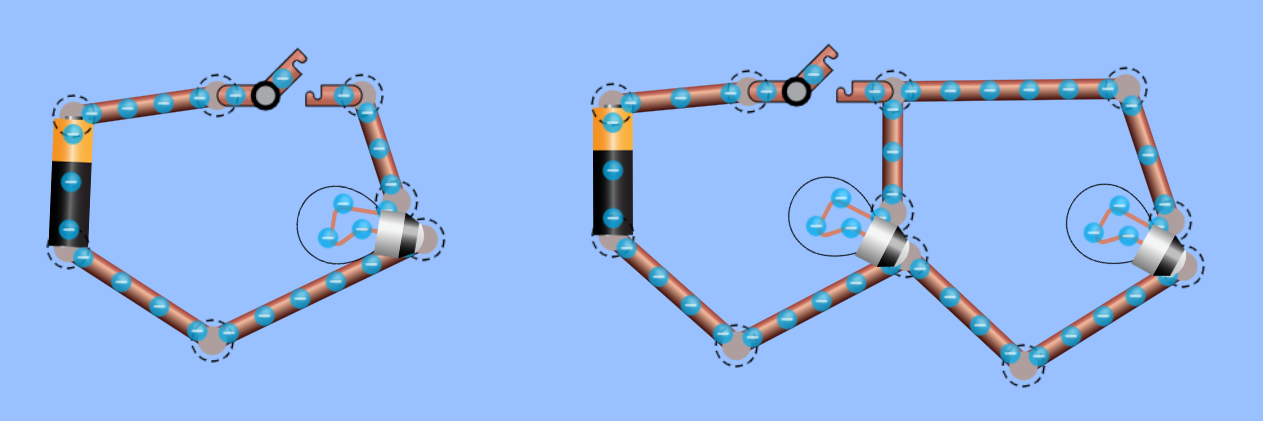
\includegraphics[width=10cm]{figures/Unit9_PhET_Circuit1.png}
\end{center}

Elements like lamps and resistors cause resistance in a circuit. \Gls{resistance} is how much a circuit element opposes the passage of electric current. The SI unit of resistance is the ohm (\qty{}{\ohm}). For example, a resistor or lamp may apply 5.0 ohms, or \qty{5.0}{\ohm}, of resistance to a circuit:

\begin{center}
\begin{circuitikz}
    \draw (0,0) to[R=\qty{5.0}{\ohm}] (2,0);
    \begin{scope}[xshift=4cm]
    \draw (0,0) to[lamp,l=\SI{5.0}{\ohm}] (2,0);
    \end{scope}
\end{circuitikz}
\end{center}

\clearpage
\subsection*{\ref{wpbAPw} Exercises}

\textbf{For the following exercises, please access the 
\phet\ Simulation called ``Circuit Construction Kit'' by \href{https://phet.colorado.edu/sims/html/circuit-construction-kit-dc/latest/circuit-construction-kit-dc_en.html}{clicking here}. Click the \texttt[red]{Intro} tab, and check the box called \texttt[red]{Labels}.}

% \begin{exercise}
%     \href{https://photos.app.goo.gl/ntKqo9sznG9w7FiUA}{Click here} to view a photo of a real-world circuit. Then use \texttt[red]{PhET} to simulation the circuit, which consists of two batteries, a switch, a lamp, and an ammeter, in series.
% \end{exercise}

\begin{exercise}
    Simulate the following circuit diagram, which is in series, in \phet . 
\end{exercise}

\begin{center}
\begin{circuitikz}
    \draw (0,0) to[lamp] (3,0) to[lamp] (3,2)
          (0,2) to[battery,l_=\qty{9.0}{V}] (0,0)
          (0,2) to[cute closed switch] (3,2);
\end{circuitikz}
\end{center}

\begin{exercise}
    On paper, draw a sketch of your \phet\ circuit. Label parts and values. 
\end{exercise}

\begin{exercise}
    Place an ammeter \textit{near} (not \textit{on}) the circuit. Use the meter to measure the current throughout all sections of wire. In your sketch, label the current through various portions of wire in the circuit.
\end{exercise}

\begin{exercise}
    Does the current change throughout the series circuit?
\end{exercise}

\begin{exercise}
    Simulate the following circuit, which contains two lamps in parallel, in \phet .
\end{exercise}

\begin{center}
\begin{circuitikz}
    \draw (0,0) -- (3,0) to[lamp] (3,2)
        (3,0) -- ++(2,0) to[lamp] ++(0,2) -- ++(-2,0)
        (0,2) to[battery,l_=\qty{9.0}{V}] (0,0)
        (0,2) to[cute open switch] (3,2);
\end{circuitikz}
\end{center}

\begin{exercise}
    On paper, draw a sketch of your \phet\ circuit. Label parts and values. 
\end{exercise}

\begin{exercise}
    Place an ammeter near the circuit. Use the meter to measure the current throughout all sections of wire. In your sketch, label the current through various portions of wire in the circuit.
\end{exercise}

\begin{exercise}
    Does the current change throughout the parallel circuit?
\end{exercise}

\begin{exercise}
    For both circuits created above, add a resistor near the battery. Re-measure the current through the wires with an ammeter. In each circuit, how did the resistor change the current through the wires?
\end{exercise}

% \begin{center}
% \begin{minipage}{0.45\textwidth}
%     \centering
%     \includegraphics[width=6cm]{figures/Unit9_Circuit1.png}
% \end{minipage}%
% \begin{minipage}{0.45\textwidth}
%     \centering
%     \includegraphics[width=6cm]{figures/Unit9_Circuit2.png}
% \end{minipage}
% \end{center}

% \begin{center}
% \begin{minipage}{0.45\textwidth}
%     \centering
%     \includegraphics[width=6cm]{figures/Unit9_Circuit3.png}
% \end{minipage}%
% \begin{minipage}{0.45\textwidth}
%     \centering
%     \includegraphics[width=6cm]{figures/Unit9_Circuit4.png}
% \end{minipage}
% \end{center}

\clearpage

\subsection{Ohm's Law} \label{nJeAQY}

Previously we defined \gls{electric current} ($I$) as electric charge that moves through wires, and \gls{resistance} ($R$) as the opposition of electric current by an element in a circuit. A third quantity is voltage.

\vspace{1em}

\Gls{voltage} ($V$) is defined as the electric potential energy per unit charge. You can think of voltage as the ``pressure or pushing force in a circuit\footnote{See ``\href{https://youtu.be/HsLLq6Rm5tU?t=291}{Ohms Law Explained}'' by The Engineering Mindset on \textit{YouTube}.}.'' It's supplied to a circuit by a battery. When current crosses an element with resistance, like a lamp or a resistor, voltage \textit{drops} across that element. Voltage is measured by connecting a voltmeter across circuit elements (batteries, resistors, etc.). The SI unit of voltage is the volt (V). 

\vspace{1em}

Next, we introduce Ohm's law, which links voltage, current, and resistance. \gls{Ohm's law} states that electric current is proportional to the voltage applied across a circuit or other path. More usefully, Ohm's law in equation form is

\begin{equation} \label{cS0E6k}
    V = IR
\end{equation}

\begin{center}
    \begin{tabular}{cl|cc}
    \hline
    \textbf{Symbol} & \textbf{Quantity} & \textbf{SI Base Unit} & \textbf{Unit Symbol}  \\
    \hline\hline
    \rule{0pt}{2.5ex}
        $V$ & voltage & volt & V\\
        $I$ & current & ampere & A\\
        $R$ & resistance & ohm & \qty{}{\ohm}\\
    \hline
    \end{tabular}
\end{center}

\cyanhrule

\begin{example}
    When a battery and 3.5-ohm resistor are connected in a circuit, the current through the wires is 0.43 amperes. What is the voltage of the battery?
\end{example}

\Solution It's good practice to draw a circuit diagram, to help you visualize the circuit:

\begin{center}
    \begin{circuitikz}
        \draw (0,2.5) to[battery,l_=$V$,i={$\SI{0.43}{A}$}] (0,0) -- (2,0) to[R,l_={$\SI{3.5}{\ohm}$}]
            (2,2.5) -- (0,2.5);
    \end{circuitikz}
\end{center}

We are given current and resistance through a series circuit: $I = \SI{0.43}{A}$ and $R = \qty{3.5}{\ohm}$. The unknown is the voltage: $V = \text{?}$ By Ohm's law (Eq.~\ref{cS0E6k}), the voltage supplied by the battery is

\begin{equation*}
    V = I R = (0.43)(3.5) = 1.5
\end{equation*}

Therefore, the battery's voltage is 1.5 volts.

\vspace{1em}

\cyanhrule

\clearpage
\begin{example}
    What is the resistance of an automobile headlight through which \SI{2.50}{A} flows when \SI{12.0}{V} is applied to it?
\end{example}

\Solution We are given the current and voltage: $I = \SI{2.50}{A}$ and $V = \SI{12.0}{V}$. The unknown is the resistance: $R =\ ?$ These quantities are related by Ohm's law (Eq.~\ref{cS0E6k}):

\begin{equation*}
    V = IR
\end{equation*}

Substituting values leads to

\begin{equation*}
    12 = 2.5\,R
\end{equation*}

We solve for resistance as follows:

\begin{align*}
    \textbf{Write $R$ on left} \qquad & 2.5\,R = 12 \\[1ex]
    \textbf{Divide by 2.5} \qquad & \frac{\cancel{2.5}\,R}{\textcolor{red}{\cancel{2.5}}} = \frac{12}{\textcolor{red}{2.5}}\\[1ex]
    \textbf{Simplify} \qquad & R = \SI{4.8}{\ohm}
\end{align*}

The resistance in the headlight is 4.8 ohms.

\vspace{1em}

\cyanhrule

\subsection*{\ref{nJeAQY} Exercises}

\setlength{\columnsep}{8mm}
\setlength{\columnseprule}{1pt}
\def\columnseprulecolor{\color{cyan}}

\begin{multicols*}{2}

\begin{exercise} \label{t0aM6F}
    Find the voltage of the battery in the circuit shown below.
\end{exercise}

\begin{center}
    \begin{circuitikz}
        \draw (0,2.5) to[battery,l_=$V$,i={$\SI{0.16}{A}$}] (0,0) -- (2,0) to[R,l_={$\SI{25}{\ohm}$}]
            (2,2.5) -- (0,2.5);
    \end{circuitikz}
\end{center}

\begin{exercise} \label{9ZzyyD}
    When a \qty{9.0}{V} battery and lamp are connected in a circuit, the resistance through the lamp is \qty{36}{\ohm}. What is the current through the lamp?
\end{exercise}

\begin{exercise} \label{x4zyhF}
    The current through a \SI{10}{\ohm} resistor 
    is \SI{0.25}{A}. What is the voltage drop across the resistor?
\end{exercise}

\begin{exercise}\label{CYRksH}
    Find the resistance of the unknown resistor shown below.
\end{exercise}

\begin{center}
    \begin{circuitikz}
        \draw (0,2.5) to[battery,l_=$\SI{4.5}{V}$,i={$\SI{0.9}{A}$}] (0,0) -- (2,0) to[R,l_={$R$}]
            (2,2.5) -- (0,2.5);
    \end{circuitikz}
\end{center}

\begin{exercise} \label{0rWTxi}
    What is the current through the lamp shown in the circuit below?
\end{exercise}

\begin{center}
    \begin{circuitikz}
        \draw (0,1.5) -- (0,0) to[lamp,l_=\qty{40}{\ohm}] (3,0) -- (3,1.5)
            to[battery,l_=\qty{8}{V},i=$I$] (0,1.5);
    \end{circuitikz}
\end{center}

\end{multicols*}


\clearpage
\subsection{Resistors in Series and Parallel} \label{TaE0On}

Consider two resistors in series or in parallel

\begin{center}
    \begin{circuitikz}
        \draw (0,0) to[R=$R_1$] (2.5,0) to[R=$R_2$] (5,0);
        \begin{scope}[xshift=7cm]
            \draw (0,0) -- (1,0) -- (1,1) to[R=$R_1$] (3,1) -- (3,0) -- (4,0)
                (1,0) -- (1,-1) to[R=$R_2$] (3,-1) -- (3,0);
        \end{scope}
    \end{circuitikz}
\end{center}

The equivalent resistance of resistors in series is

\begin{equation} \label{E2hx8w}
    R_{\mathrm{eq}} = R_1 + R_2
\end{equation}

For resistors in parallel, equivalent resistance is 

\begin{equation} \label{nxHaL8}
    R_{\mathrm{eq}} = \left(\frac{1}{R_1} + \frac{1}{R_2}\right)^{-1}
\end{equation}

\subsection*{\ref{TaE0On} Exercises}

\begin{multicols*}{2}
    


\begin{exercise} \label{z25jPn}
    \phantom{.}
    \begin{center}
        \tikz \draw (0,0) to[R=$\SI{17}{\ohm}$] (3,0) to[R=$\SI{71}{\ohm}$] (6,0);
    \end{center}
\end{exercise}

\begin{exercise} \label{NRON6F}
    \phantom{.}
    \begin{center}
        \tikz \draw (0,0) -- (1,0) -- (1,1) to[R=\SI{47}{\ohm}] (3,1) -- (3,0) -- (4,0)
        (1,0) -- (1,-1) to[R=\SI{75}{\ohm}] (3,-1) -- (3,0);
    \end{center}
\end{exercise}

\begin{exercise} \label{x7ZMs2}
    \phantom{.}
    \begin{center}
        \tikz \draw (0,0) to[R=\SI{22}{\ohm}] (3,0) to[R=\SI{56}{\ohm}] (6,0);
    \end{center}
\end{exercise}

\begin{exercise} \label{2QgW9g}
    \phantom{.}
    \begin{center}
        \tikz \draw (0,0) -- (1,0) -- (1,1) to[R=\SI{5}{\ohm}] (3,1) -- (3,0) -- (4,0)
        (1,0) -- (1,-1) to[R=\SI{86}{\ohm}] (3,-1) -- (3,0);
    \end{center}
\end{exercise}


\begin{exercise} \label{xjuTz7}
    \phantom{.}
    \begin{center}
        \tikz \draw (0,0) to[R=\SI{33}{\ohm}] (3,0) to[R=\SI{86}{\ohm}] (6,0);
    \end{center}
\end{exercise}

\begin{exercise} \label{MEfjff}
    \phantom{.}
    \begin{center}
        \tikz \draw (0,0) -- (1,0) -- (1,1) to[R=\SI{150}{\ohm}] (3,1) -- (3,0) -- (4,0)
        (1,0) -- (1,-1) to[R=\SI{101}{\ohm}] (3,-1) -- (3,0);
    \end{center}
\end{exercise}
\end{multicols*}

\clearpage

\subsection{Current in Series and Parallel} \label{GheYvY}

\begin{example} \label{0Jjx1M}
Go to the ``Circuit Construction Kit'' \phet (\href{https://phet.colorado.edu/sims/html/circuit-construction-kit-dc/latest/circuit-construction-kit-dc_en.html}{click here}). In \phet, build the following circuit, which contains two resistors in parallel. Use an ammeter to measure and record electric currents through all sections of wire. Using markers of different colors, highlight the entire section of wire if the current through that section is constant. Label the magnitude of current, in amperes, through each section.

\begin{center}
    \begin{circuitikz}
        \draw (3,4) -- (0,4) to[battery,l=\SI{12}{V}] (0,0) -- (3,0);
        \draw (3,4) to[R=\SI{3.0}{\ohm}] (3,0);
        \draw (3,4) -- (5,4) to[R=\SI{8.0}{\ohm}] (5,0) -- (3,0);
    \end{circuitikz}
\end{center}
\end{example}

\Solution When using the ammeter to measure current throughout different portions of wire, we see that there are 3 constant currents throughout the circuit: \SI{1.50}{A}, \SI{4.00}{A}, and \SI{5.50}{A}:

\vspace{1em}

\begin{minipage}{0.45\textwidth}
    \centering
    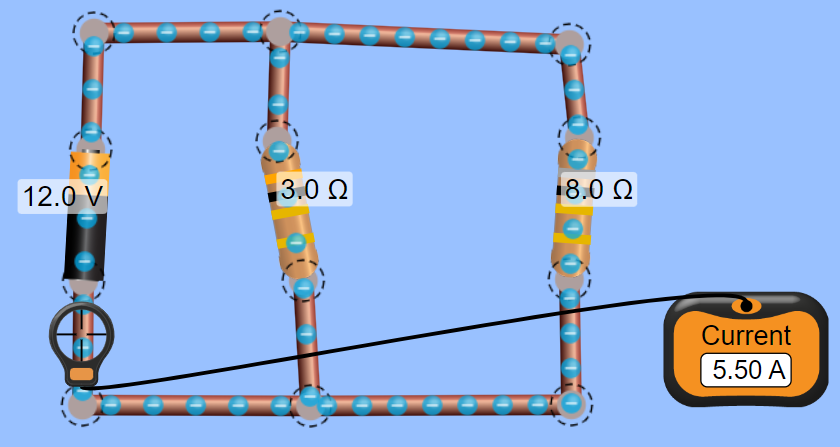
\includegraphics[width=7cm]{figures/Unit9_PhET_Circuit2.png}
\end{minipage}%
\hspace{10mm}
\begin{minipage}{0.45\textwidth}
    \centering
    \begin{circuitikz}
        \draw[Green,thick] (3,0) -- (0,0) to[battery,color=Green,l=\SI{12}{V}, i=\SI{5.50}{A}] (0,4) -- (3,4);
        \draw[red,thick] (3,0) to[R,l_=\SI{3.0}{\ohm},color=red,i_=\SI{4.00}{A}] (3,4);
        \draw[blue,thick] (3,0) -- (5,0) to[R,l_=\SI{8.0}{\ohm},color=blue,i_=\SI{1.50}{A}] (5,4) -- (3,4);
    \end{circuitikz}
\end{minipage}

\vspace{1em}

\cyanhrule

\begin{example}
    For the circuit in Example \ref{0Jjx1M}, use Ohm's law, in the \textit{absence} of an ammeter, to calculate the currents through each element.
\end{example}

\Solution Recall that Ohm's law relates voltage, current, and resistance as

\begin{equation*}
    V = I R
\end{equation*}

which implies that current is

\begin{equation*}
    I = \frac{V}{R}
\end{equation*}

In this circuit, the voltage drop across all components (battery and 2 resistors) is the voltage of the battery: 12 volts. The current through the first resistor is

\begin{equation*}
        I_1 = \frac{V}{R_1} = \frac{\SI{12}{V}}{\SI{3.0}{\ohm}} =  \SI{4.00}{A}
\end{equation*}

Current through the second resistor is

\begin{equation*}
    I_2 = \frac{V}{R_2} = \frac{\SI{12}{V}}{\SI{8.0}{\ohm}} = \SI{1.50}{A}
\end{equation*}

To find the current through the battery, we first need to calculate the equivalent resistance of the two resistors in parallel, using Equation \ref{nxHaL8}:

\begin{equation*}
    R_{\mathrm{eq}} = \left(\frac{1}{R_1} + \frac{1}{R_2}\right)^{-1} = \left(\frac{1}{3} + \frac{1}{8}\right)^{-1} = \SI{2.18}{\ohm}
\end{equation*}

Therefore, current through the battery is

\begin{equation*}
    I = \frac{V}{R_{\text{eq}}} = \frac{\SI{12}{V}}{\SI{2.18}{\ohm}} = \SI{5.50}{A}
\end{equation*}

\cyanhrule

\subsection*{\ref{GheYvY} Exercises}

For each of the circuits below, calculate the three currents flowing through the wires. Draw a quick sketch, and label those currents on the sketch.

\begin{exercise} \label{Vr76KR}
    \phantom{.}
\end{exercise}

\begin{center}
    \begin{circuitikz}
        \draw (3,3) -- (0,3) to[battery,l=\SI{9}{V}] (0,0) -- (3,0);
        \draw (3,3) to[R=\SI{44}{\ohm}] (3,0);
        \draw (3,3) -- (5,3) to[R=\SI{77}{\ohm}] (5,0) -- (3,0);
    \end{circuitikz}
\end{center}

\begin{exercise} \label{wlE3QV}
    \phantom{.}
\end{exercise}

\begin{center}
    \begin{circuitikz}
        \draw (3,3) -- (0,3) to[battery,l=\SI{15}{V}] (0,0) -- (3,0);
        \draw (3,3) to[R=\SI{55}{\ohm}] (3,0);
        \draw (3,3) -- (5,3) to[R=\SI{80}{\ohm}] (5,0) -- (3,0);
    \end{circuitikz}
\end{center}

\begin{exercise} \label{XhaPdx}
    \phantom{.}
\end{exercise}

\begin{center}
    \begin{circuitikz}
        \draw (3,3) -- (0,3) to[battery,l=\SI{9}{V}] (0,0) -- (3,0);
        \draw (3,3) to[R=\SI{9.0}{\ohm}] (3,0);
        \draw (3,3) -- (5,3) to[R=\SI{37}{\ohm}] (5,0) -- (3,0);
    \end{circuitikz}
\end{center}








% \vspace{1em}

% \begin{circuitikz}
% \draw (0,3) to[battery, l=$V$,i=$I$] (0,0) -- (2,0)
% to[R=$R_2$] (2,3) -- (0,3);
% \draw (2,3) -- (4,3) to[R=$R_2$]
% (4,0) -- (2,0);
% \end{circuitikz}

% \begin{circuitikz}
% \draw (0,3) to[battery,l=$V$,i=$I$] (0,0);
% \draw (0,3) to[R=$R_1$] (3,3)
%     to[R=$R_2$] (3,0)
%     to[R=$R_3$] (0,0);
% \end{circuitikz}

\clearpage

\subsection{Voltage in Series and Parallel}

\begin{example}
    What is the voltage measured by the voltmeter across the resistor in the circuit below?

    \vspace{1em}
    
\begin{center}
\begin{circuitikz}
    \draw (0,0) -- (3,0) to[R=\SI{15}{\ohm}] ++(0,3) to[R=\SI{10}{\ohm}] ++(-3,0) to[battery,l=\SI{9.0}{V}] (0,0)
            (0.5,3) -- ++(0,1) to[rmeter,t=V] ++(2,0) -- ++(0,-1);
\end{circuitikz}
\end{center}

\end{example}

\Solution
To calculate the voltage through the 10-ohm resistor, we need to know the current through it. Since this circuit is in series, the same current runs through the whole circuit. This current is found be considering the equivalent resistance:

\begin{center}
\begin{circuitikz}
    \draw (0,0) -- (3,0) to[R,l_=$R_{\mathrm{eq}}$] ++(0,3) -- ++(-3,0) to[battery,l=\SI{9.0}{V}] (0,0)
            (0.5,3);
\end{circuitikz}
\end{center}

where equivalent resistance is, by Eq.~(\ref{E2hx8w}),

\begin{equation*}
    R_{\mathrm{eq}} = R_1 + R_2 = \SI{10}{\ohm} + \SI{15}{\ohm} = \SI{25}{\ohm}
\end{equation*}

The voltage of the battery is $V = \SI{9.0}{V}$, and the current through the circuit, by Ohm's law ($V = I R$), is

\begin{equation*}
    I = \frac{V}{R_{\text{eq}}} = \frac{\SI{9}{V}}{\SI{25}{\ohm}} = \SI{0.36}{A}
\end{equation*}

This 0.36-ampere current runs through the 10-ohm resistor, so the voltage across that resistor is

\begin{equation*}
    V = IR = (0.36)(10) = \SI{3.6}{V}
\end{equation*}

Therefore, the voltmeter reads 3.6 volts.

\vspace{1em}

\cyanhrule

\clearpage

\subsection*{Exercises}

Calculate the voltage measured by the voltmeter in each of the circuits below.

\begin{exercise} \label{m9FFN5}
\phantom{.}

\begin{center}
\begin{circuitikz}
    \draw (0,0) -- (3,0) to[R=\SI{15}{\ohm}] ++(0,3) to[R=\SI{10}{\ohm}] ++(-3,0) to[battery,l=\SI{9.0}{V}] (0,0)
            (0.5,3);
    \draw (3,2.5) -- ++(1,0) to[rmeter,t=V] ++(0,-2) -- ++(-1,0);
\end{circuitikz}
\end{center}

\end{exercise}

\begin{exercise} \label{mLtImA}
\phantom{.}

\begin{center}
\begin{circuitikz}
    \draw (0,0) -- (3,0) to[R=\SI{25}{\ohm}] ++(0,3) to[R=\SI{75}{\ohm}] ++(-3,0) to[battery,l=\SI{60}{V}] (0,0)
            (0.5,3) -- ++(0,1) to[rmeter,t=V] ++(2,0) -- ++(0,-1);
\end{circuitikz}
\end{center}
\end{exercise}

\begin{exercise} \label{49hnUx}
\phantom{.}

\begin{center}
\begin{circuitikz}
    \draw (0,0) -- (3,0) to[R=\SI{18}{\ohm}] ++(0,3) to[R=\SI{24}{\ohm}] ++(-3,0) to[battery,l=\SI{15}{V}] (0,0)
            (0.5,3);
    \draw (3,2.5) -- ++(1,0) to[rmeter,t=V] ++(0,-2) -- ++(-1,0);
\end{circuitikz}
\end{center}

\end{exercise}



\clearpage
\subsection*{Answers to Select Exercises}

\ref{t0aM6F}. \SI{4.0}{V}\\
\ref{9ZzyyD}. \SI{0.25}{A}\\
\ref{x4zyhF}. \SI{2.5}{V}\\
\ref{CYRksH}. \SI{5.0}{\ohm}\\
\ref{0rWTxi}. \SI{0.2}{A}\\
\ref{z25jPn}. \SI{88}{\ohm}\\
\ref{NRON6F}. \SI{28.9}{\ohm}\\
\ref{x7ZMs2}. \SI{78}{\ohm}\\
\ref{2QgW9g}. \SI{4.72}{\ohm}\\
\ref{xjuTz7}. \SI{119}{\ohm}\\
\ref{MEfjff}. \SI{60.4}{\ohm}\\
\ref{Vr76KR}. \SI{0.20}{A}, \SI{0.11}{A}, \SI{0.32}{A}\\ 
\ref{wlE3QV}. \SI{0.27}{A}, \SI{0.19}{A}, \SI{0.46}{A}\\ 
\ref{XhaPdx}. \SI{1.0}{A}, \SI{0.24}{A}, \SI{1.24}{A}\\ 
\ref{m9FFN5}. \SI{5.4}{V}\\
\ref{mLtImA}. \SI{45}{V}\\
\ref{49hnUx}. \SI{6.4}{V}\\


% \clearpage
\subsection*{Additional Resources}

``Ohms Law Explained'' by \texttt{The Engineering Mindset} on \textit{YouTube} (\href{https://youtu.be/HsLLq6Rm5tU}{click here})

\textit{YouTube}: ``Resistors in Series and Parallel'' by \texttt{Ben Finio} 
(\href{https://youtu.be/bTnQUZ4Hi-E}{click here})

\clearpage
\printnoidxglossaries


\end{document}

\begin{tabular}{|m{0.25\textwidth}|m{0.7\textwidth}|}
    \hline  
    \cellcolor{black!20}\textbf{Date} &
    \cellcolor{black!20}\textbf{Day 2023} \\
    \hline
    Learning Intention (TPO) &  \\
    \hline
    Hook/Warm Up/Opening & \\
    \hline
    Lesson/Learning Activities & \\
    \hline
    Graded Activities & \\
    \hline
    Closure & \\  
    \hline
\end{tabular}  

%%%%%%%%%%%%%%%%%%%%%%%%%%%%%%%%%%%%%%%%%%%%%%%%%%%%%%%%%

\begin{example}
    A rain cloud discharges 100 billion billion excess electrons through a lightning strike. What is the total charge carried by the lightning strike?
\end{example}

\Solution We are given the number of excess electrons:

\begin{equation*}
    n = \text{100 billion billion} = 100 \times 10^9 \times 10^9 = 100 \times 10^{18}
\end{equation*}

or simply just $10^{20}$ electrons. The charge on just \textit{one} electron is the negative elementary charge: $-e = \qty{-1.602e-19}{C}$. Therefore, the charge carried by the lightning is 100 billion billion times $-e$:

\begin{equation*}
    q = - n e = -(100 \times 10^{18}) \times \left(\qty{1.602e-19}{}\right) = \qty{-16}{C}
\end{equation*}